\section{Results}
We implemented our algorithm in C++ using Eigen\cite{eigenweb} for linear algebra routines. We run our experiments on a desktop with a 4-core Intel i7  processor clocked at 4 GHz and 32 GB of memory, but using only one thread on a single core.
For all experiments, the scaffold bounding box is computed by uniformly scaling by three times the bounding box of the image of the current map. 

\begin{figure}[t]
\centering
\includegraphics[width=8cm]{scaf-tex/figs/database_demo}
\caption{Two models are cut using \cite{Bommes:2009} and bijectively parametrized using our algorithm. See the additional material for more examples.}
\label{scaf:fig:miq_database}
\vspace{-0.2cm}
\end{figure}

\paragraph{Robustness.} To demonstrate the robustness of our algorithm, we computed  bijective maps for all the 102 meshes parametrized by the MIQ algorithm \cite{Bommes:2009} and for the 17 meshes parametrized by  \cite{Myles:2014} in the dataset proposed by \cite{Myles:2014}. The cuts in these meshes have been designed for locally injective parametrization that usually have major self-overlap. We use them as a stress test for the effectiveness and robustness of our method:  the cuts introduce a massive distortion in the Tutte initialization and lead to boundaries that are prone to overlap in hundreds of locations. Our method successfully creates bijective parametrizations for all these models with default parameters. We attach all the parametrized models in the additional material and show two examples in Figure \ref{scaf:fig:miq_database}. 


\paragraph{Scalability.} Our methods scales gracefully to large datasets, similarly to \cite{rabinovich2017scalable}. We repeat their scalability experiment, but producing bijective maps instead of just locally injective maps (Figure \ref{scaf:fig:scalability}). The behaviour is remarkably similar --- the density of the model (and consequently of the scaffold) does not affect the number of required iterations. 

\begin{figure}[t]
\centering
\includegraphics[width=\columnwidth]{scaf-tex/figs/lucy-scalability}
\caption{We compare the distortion energy with respect to the number of iterations on a set of Lucy's meshes with different resolutions (from 1 to 12 million faces). In the center of the plot, we show the 1M Lucy model parametrized by our algorithm.
}
\label{scaf:fig:scalability}
\end{figure}

\paragraph{Texture Atlas Generation} 

UV mapping is a time consuming procedure required in most geometric modeling pipelines. Existing commercial tools provide the ability to flatten single patches and arrange them in UV layouts where multiple patches are tightly packed inside a rectangular domain, which is then loaded in the texture memory of a GPU. 

Our algorithm can bijectively parameterize a single patch (Figure \ref{scaf:fig:manuallycut}), avoiding the typical manual UV postprocessing required with traditional tools.  Our algorithm can also be used to create automatic UV charts of models with multiple connected components (or predefined cut edges). We show an example in Figure \ref{scaf:fig:packing2D} where we detected the connected components, bijectively map the patches into a set of circles (using a grid layout), and reduce their distortion using our algorithm. The result is a tight and automatic packing without resorting to any user-interaction. Additional interactive tools can further improve the atlas by dragging\&dropping regions or translating islands while ensuring that no overlaps are introduced (Figure \ref{scaf:fig:teaser}). We show interactive sessions using our packing tool in the additional material.

\begin{figure}[t]
\centering
\includegraphics[width=8cm]{scaf-tex/figs/the_animal}
\caption{A mesh is cut by an artist into a single chart and parametrized using SLIM \protect\cite{rabinovich2017scalable} (left) and with our algorithm (right). Note that local-injectivity is not sufficient for this model, since the global overlaps in the highlighted region prevent this parametrization from being a UV texture map. Our result (right) is guaranteed to be bijective.}
\label{scaf:fig:manuallycut}
\vspace{-0.2cm}
\end{figure}

\begin{figure}[t]
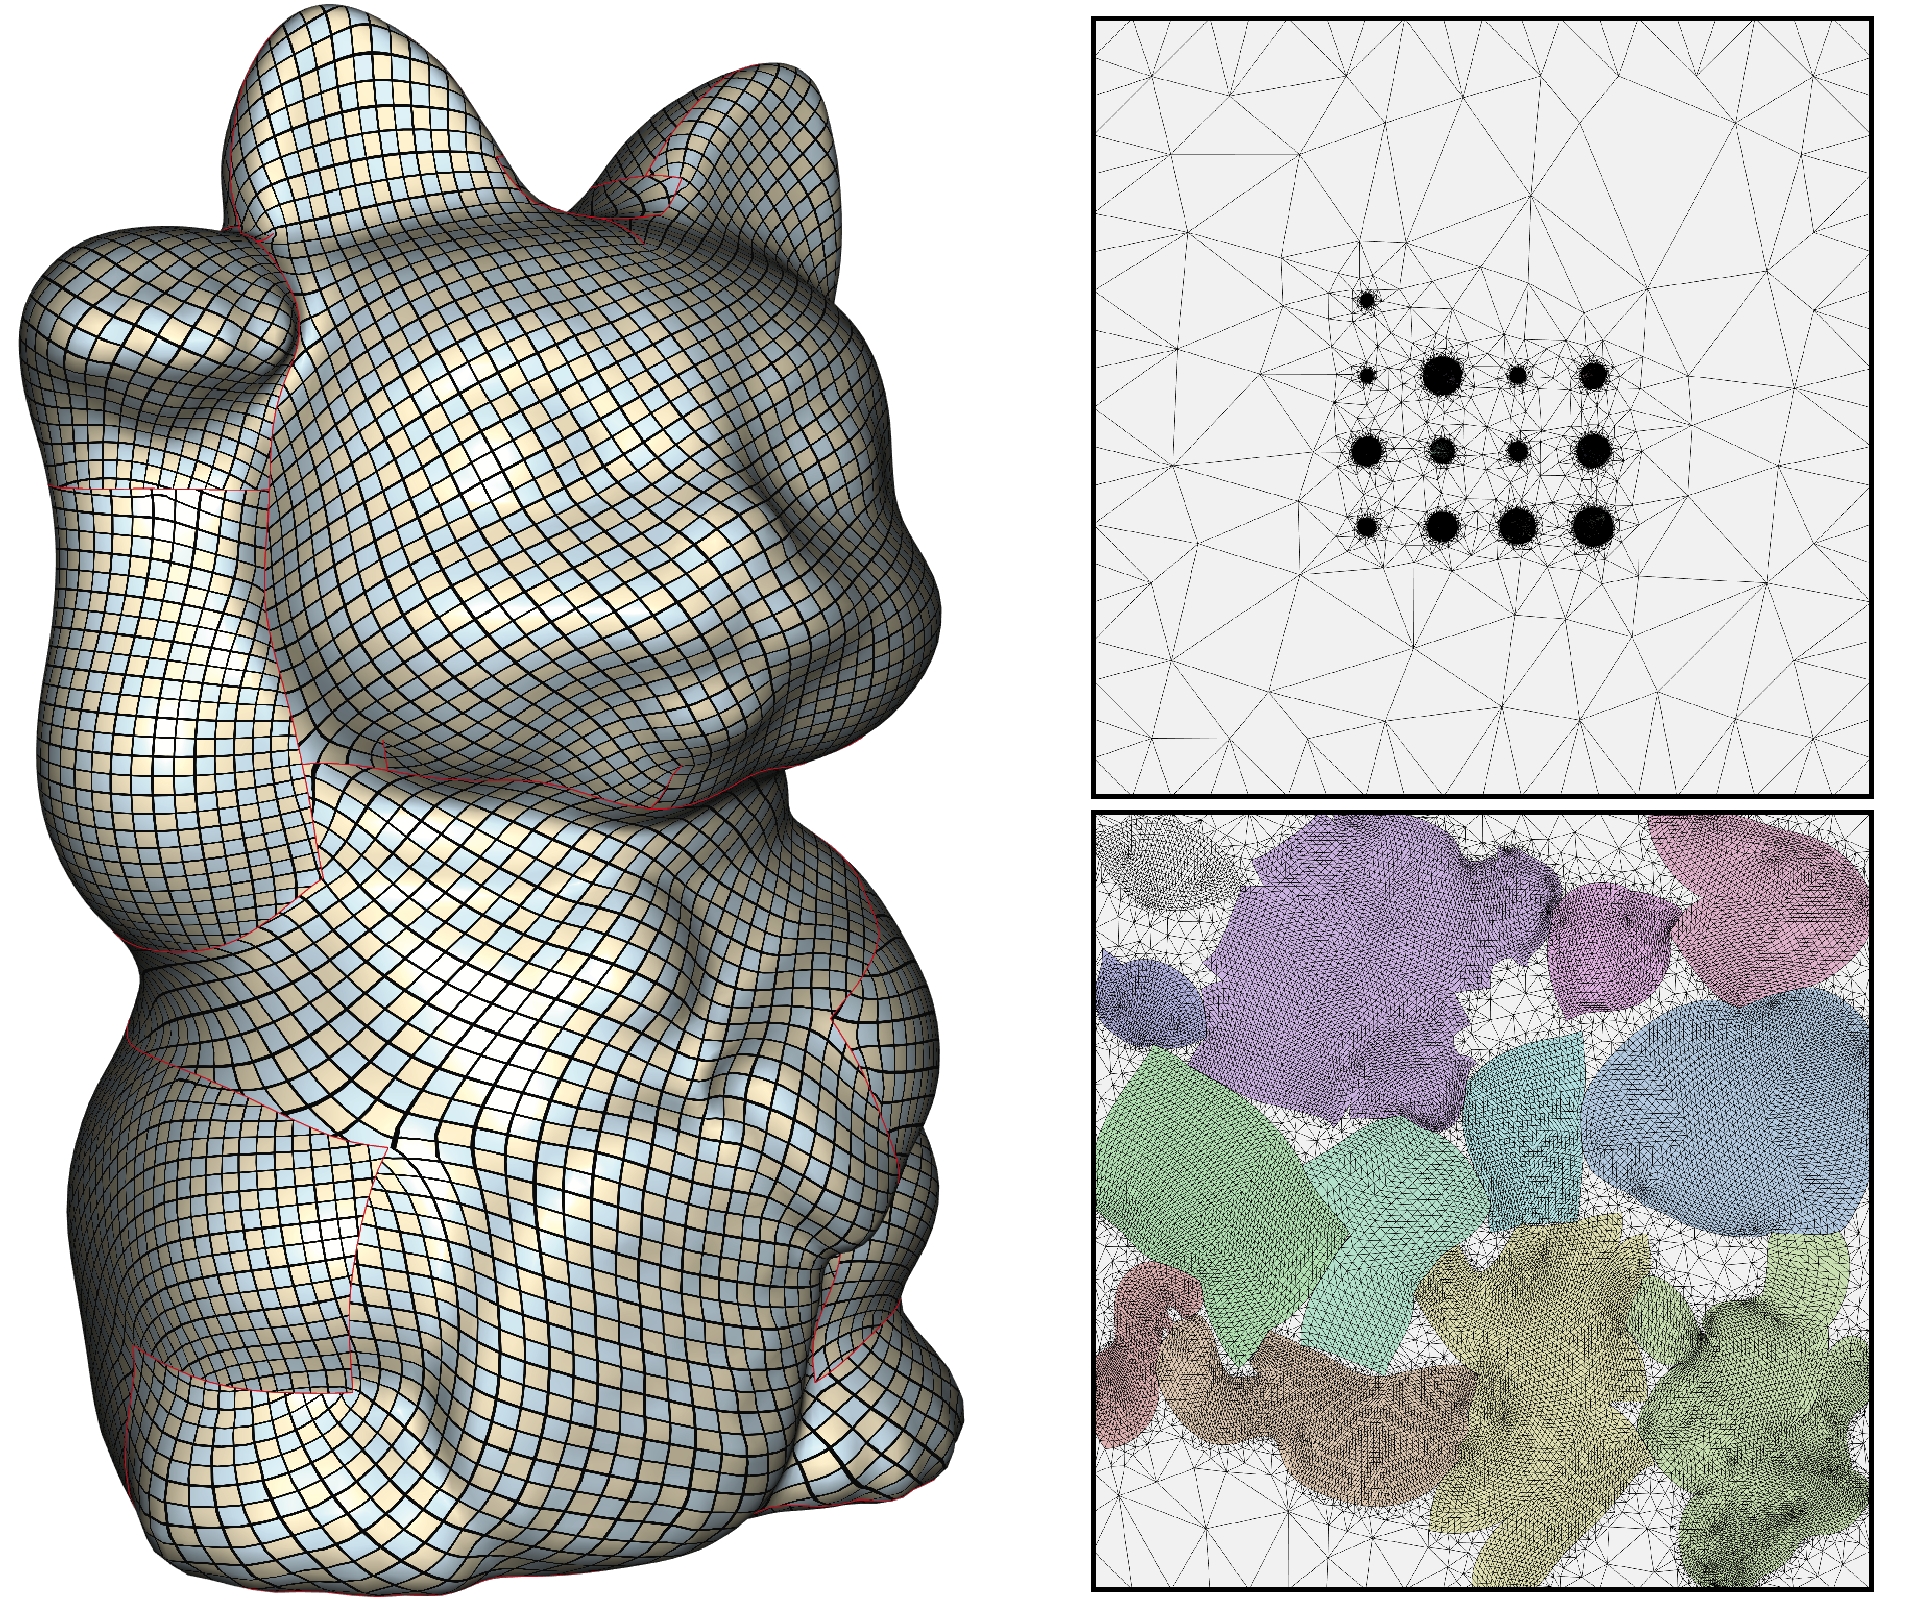
\includegraphics[width=\columnwidth]{scaf-tex/figs/maneki_neko_colorful}
\caption{A model with multiple chart (left) is automatically parametrized in a texture atlas (bottom-right) by first mapping each component to a circle (top-right) and then minimizing the distortion.}
\label{scaf:fig:packing2D}
\end{figure}

\paragraph{Preventing Self-Intersections}
Our algorithm can be generalized to handle mixed dimension problems, such as the deformation of 2D surface in 3D space, while preventing self-intersections. In Figure \ref{scaf:fig:flow}, we demonstrate the use of our method to resolve self-intersections of surfaces. First we perform a conformalized flow \cite{Kazhdan:2012} using the algorithm proposed in \cite{Sacht:2013} to resolve any self-intersections.  While \cite{Sacht:2013} will resolve the intersections, the resulting surface may be geometrically far from the initial shape (see Figure \ref{scaf:fig:flow}).  Next we tetrahedralize the ambient space while conforming to the deformed surface mesh and minimize Equation \ref{eq:variational} with an additional energy term that strives to restore the rest pose geometry of the surface, using the surface ARAP energy proposed in \cite{Sorkine:2007}. The result is a surface similar to the original mesh, but without self-intersections. In this example, it is possible to observe that even dramatic changes of scale (on the foot) can be robustly handled by our parametrization algorithm.

\begin{figure}[t]
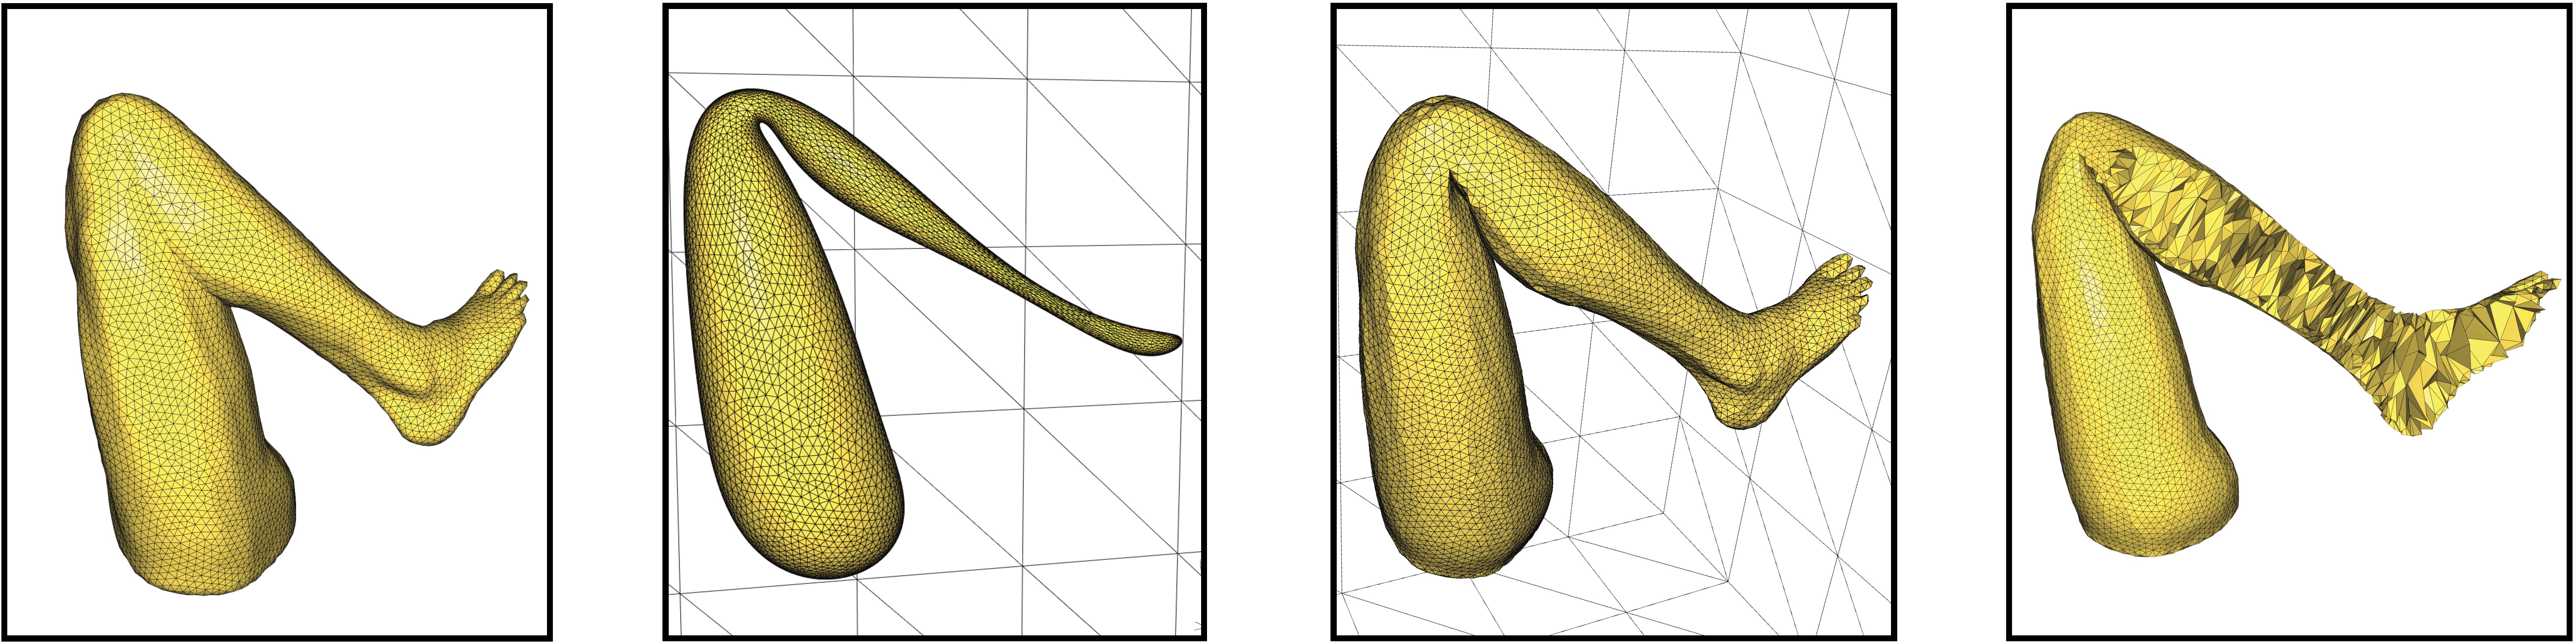
\includegraphics[width=\columnwidth]{scaf-tex/figs/leg-flow}
\caption{We remove the self-intersections from a genus 0 model using the conformalized flow \protect\cite{Kazhdan:2012,Sacht:2013}. The flow is inverted, while using our algorithm to compute a bijective volumetric map, to recover a self-intersection free version of the original surface. The final model can now be meshed using TetGen, since it is free from self-intersections.}
\vspace{-0.2cm}
\label{scaf:fig:flow}
\end{figure}

\begin{figure}[t]
\centering
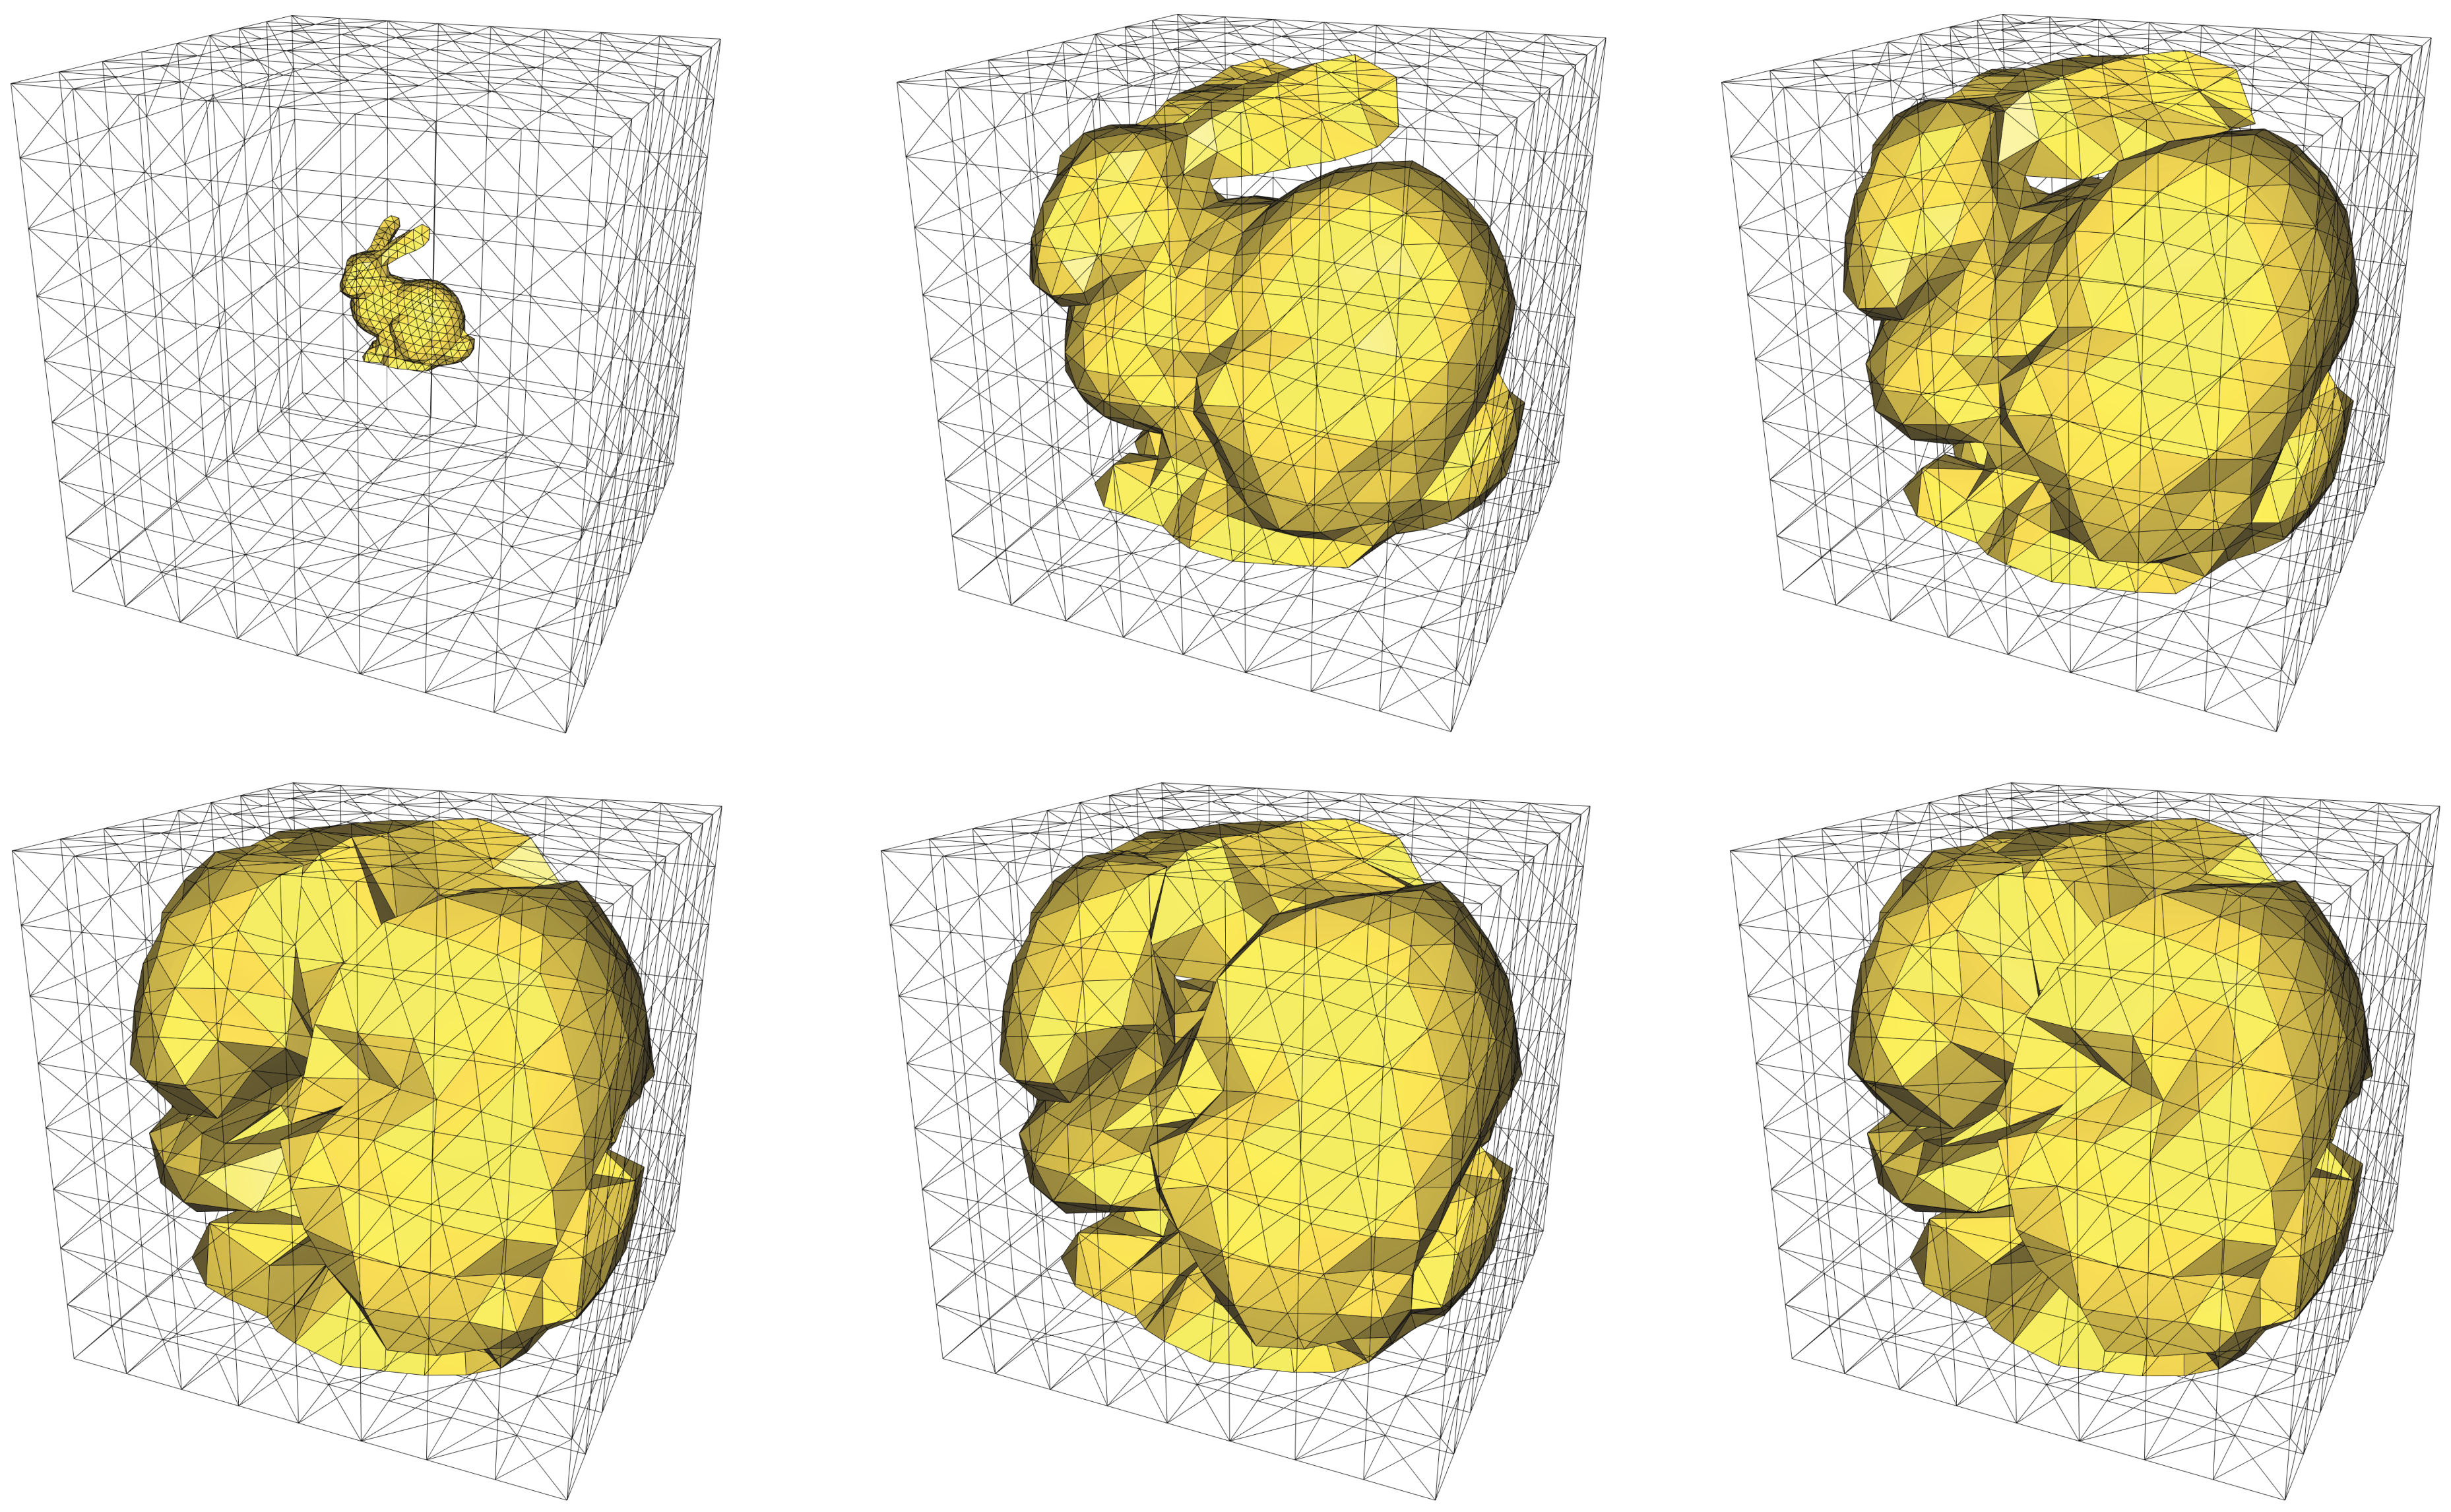
\includegraphics[width=0.8\columnwidth]{scaf-tex/figs/rabbit_grow}
\caption{We grow a bunny inside a box, while preventing  self-intersections. We show the result after 0,10,20,30,40, and 50 iterations.}
\label{scaf:fig:rabbit}
\end{figure}


A more challenging stress test is shown in Figure \ref{scaf:fig:rabbit}, where the bunny model is scaled up inside a box, to 30 times its original size. No self-intersections are introduced, despite the extreme, constrained deformation.

\paragraph{Comparison with \cite{Smith:2015}}
The algorithm closest to ours is \cite{Smith:2015}, which tackles a similar problem (restricted to the 2D case). We replicated the space filling curve experiment and obtained remarkably similar results, where our running time is 96s, compared with 8,472s for \cite{Smith:2015} (88 times faster). We show in Figure \ref{scaf:fig:smith} a more challenging experiment with a subdivided version of the space filling curve to emphasize the performance difference: our algorithm converges in 39 minutes, while \cite{Smith:2015} did not converge after 5 days and 21 hours. For this example, we used the procedure suggested in \cite{rabinovich2017scalable}: we performed a few iterations minimizing the quadratic proxy and then switch to a traditional newton method until numerical convergence. A video of the optimization is provided in the additional material.

\begin{figure}[t]
\centering
\includegraphics[width=\columnwidth]{scaf-tex/figs/dense_hilbert}
\caption{{We repeat the challenging test in \cite{Smith:2015} with a subdivided version of their Hilbert curve to increase the triangle count. Our method starts from a disc (upper left), gracefully extends (upper right), and reaches the same minimum (lower left) in 39 minutes whereas \cite{Smith:2015} didn't terminate more than 5 days (lower right), highlighting our performance boost of over 200 times.
}}
\label{scaf:fig:smith}
\vspace{-0.2cm}
\end{figure}

\begin{figure}[t]
\centering
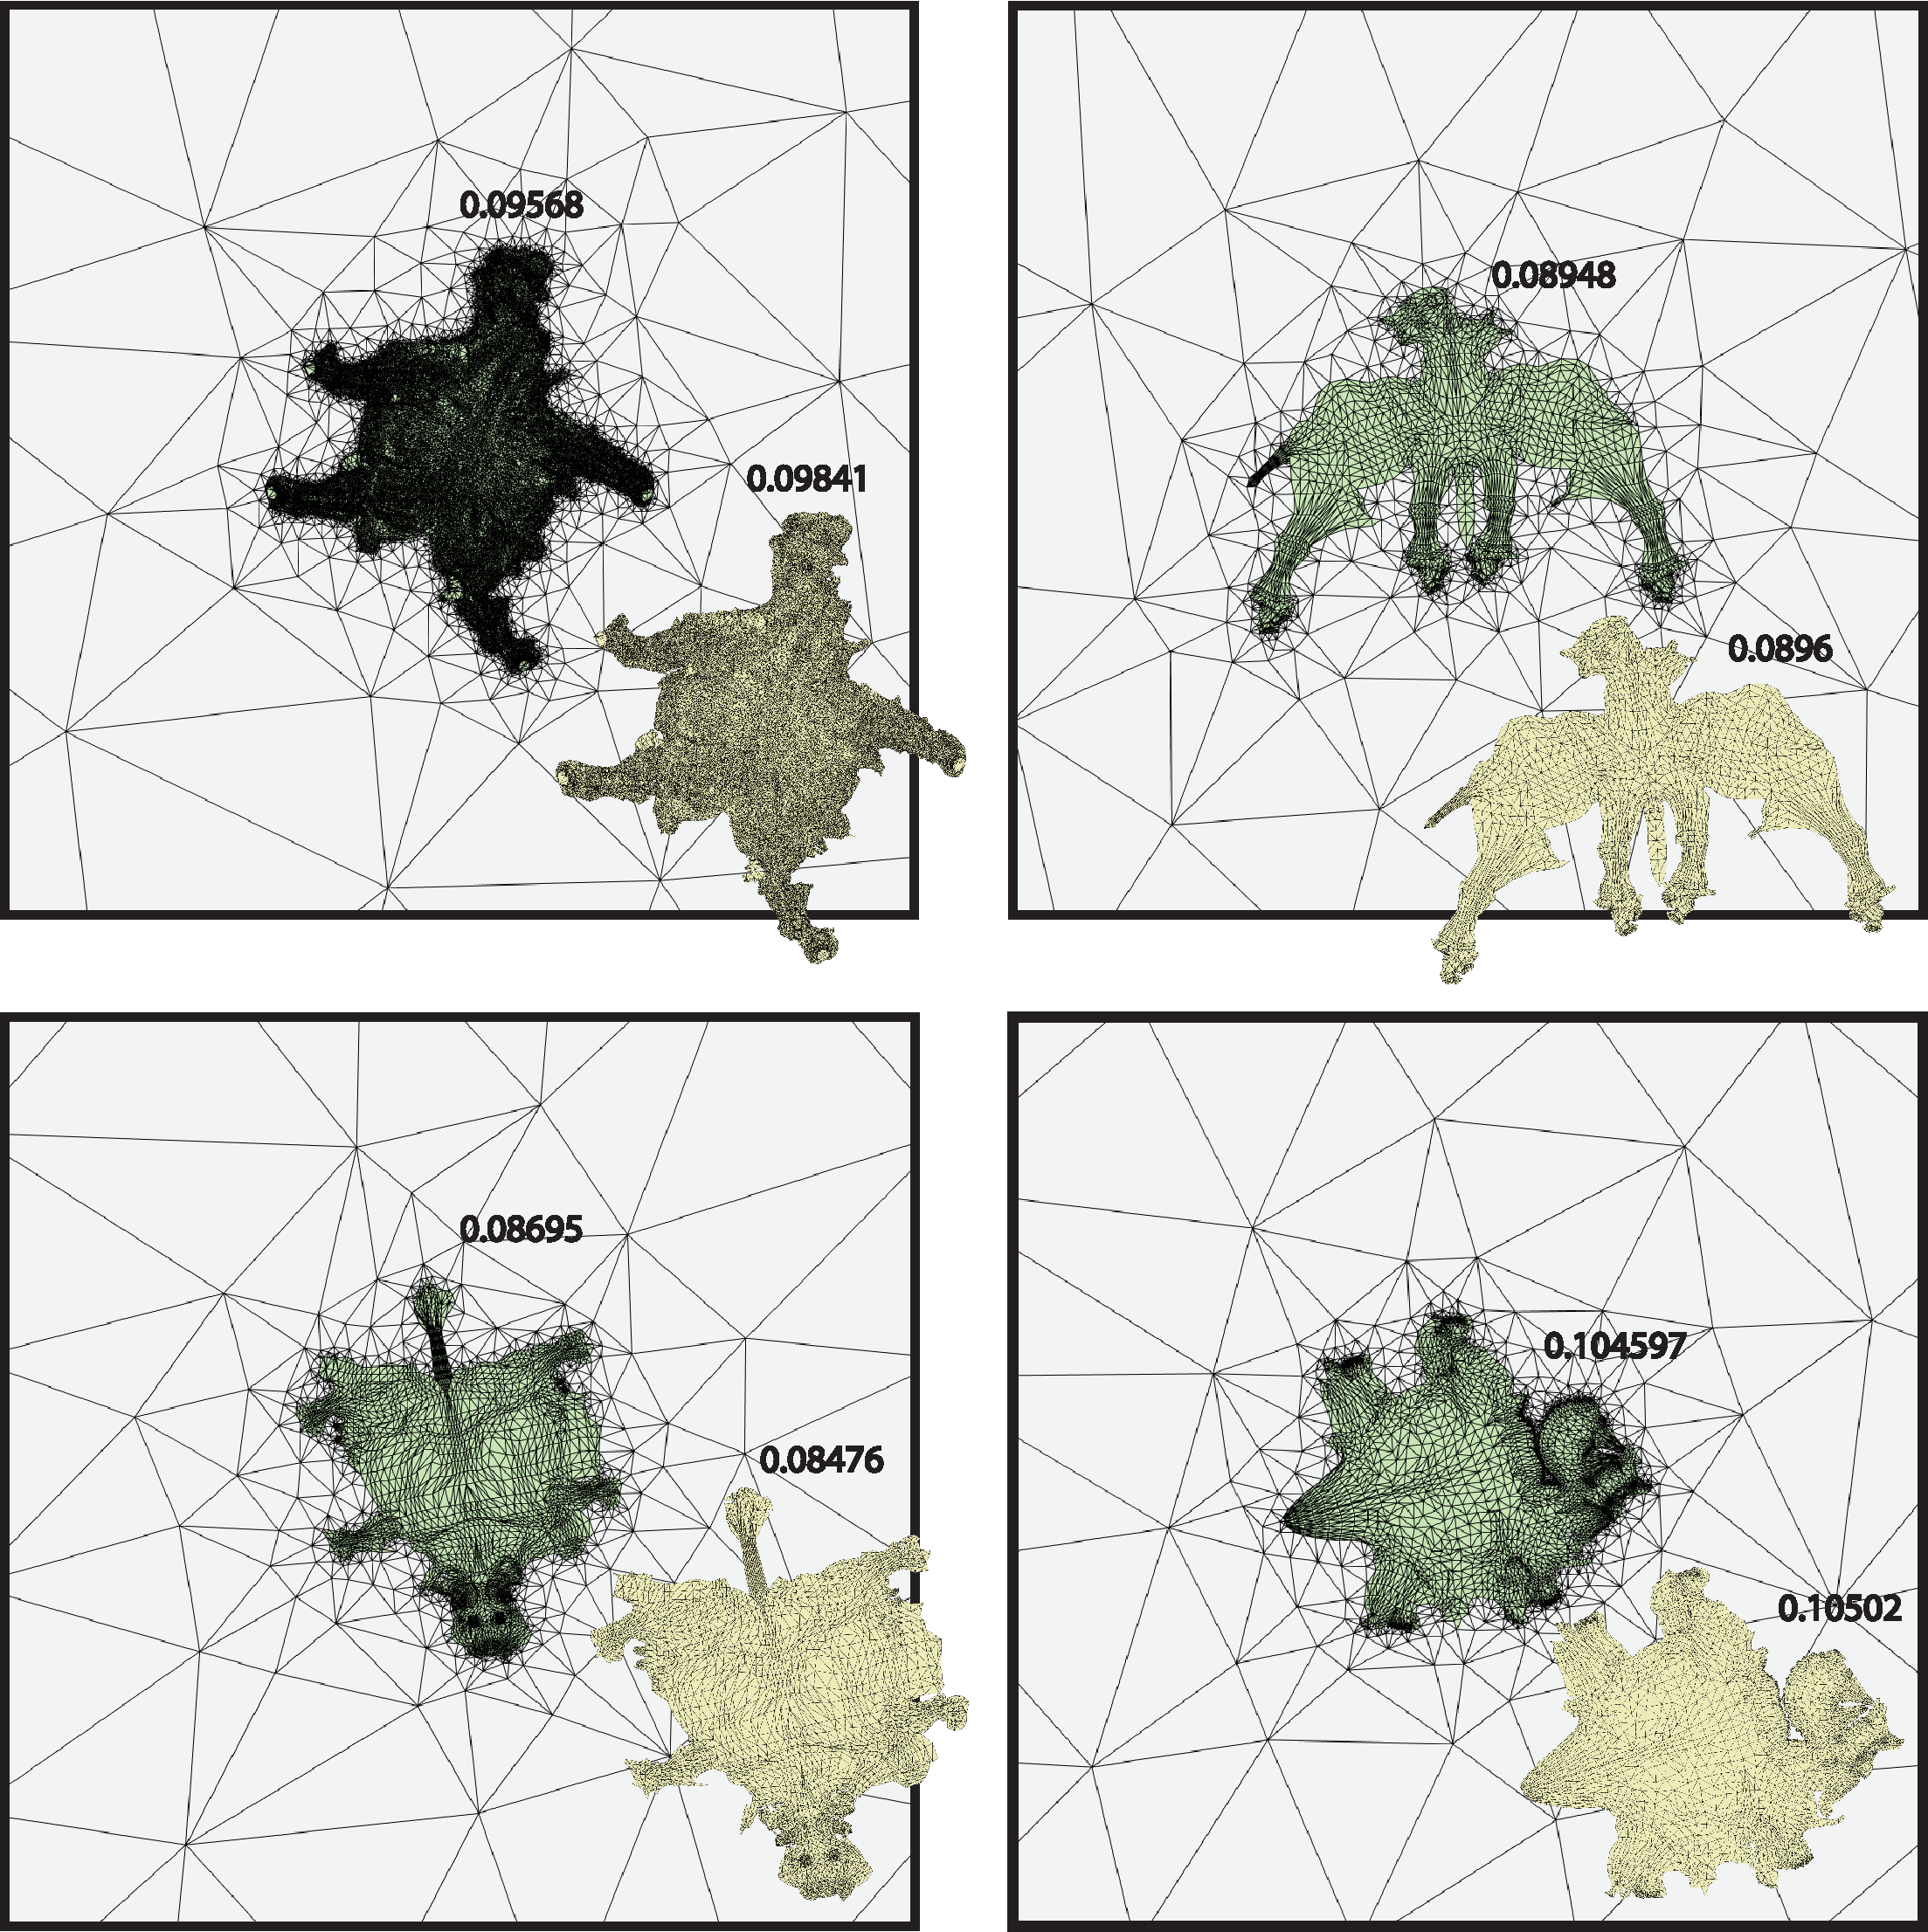
\includegraphics[width=\columnwidth]{scaf-tex/figs/compare_smith}
\caption{{We apply our algorithm on 4 models used in \cite{Smith:2015} (using the same stopping criteria) obtaining visually identical results. Distortion errors produced by our algorithm (outer) and theirs (inner) are shown in black.
}}
\label{scaf:fig:smith-all}
\vspace{-0.2cm}
\end{figure}

{Our method produces results that are visually identical to \cite{Smith:2015}. In Figure  \ref{scaf:fig:smith-all} we repeat the experiments shown in \cite{Smith:2015}, stopping our optimization at the same energy value.}

\paragraph{Local vs Global Optimization} 

Both \cite{Zhang:2005} and \cite{Misztal:2012} use a construction similar to ours to generate bijective maps (Section \ref{sec:related}). Both methods explicitly prevent changes of orientation using a local approach: they optimize the map using coordinate descent iterations \cite{SolomonBook} allowing only one vertex at a time to move in its 1-ring and thus ensuring that no triangle flip. This strategy severely limits the maximal displacement per iteration and restricts the step to the size of the 1-rings. Such a restriction makes these methods impractical for parametrization applications since the difference in scale between the Tutte's embedding and the final result is extreme (the ratio of min and max triangle area is $10^{-6}$ in Figure \ref{scaf:fig:largestep}). We show an example of one of our iterations in Figure \ref{scaf:fig:largestep}, where the highlighted vertex traversed a distance of ~150 times the size of the average edge length of its 1-ring in one single step. Using coordinate descent would have required hundreds of iterations to achieve the same effect. 

\begin{figure}[t]
\centering
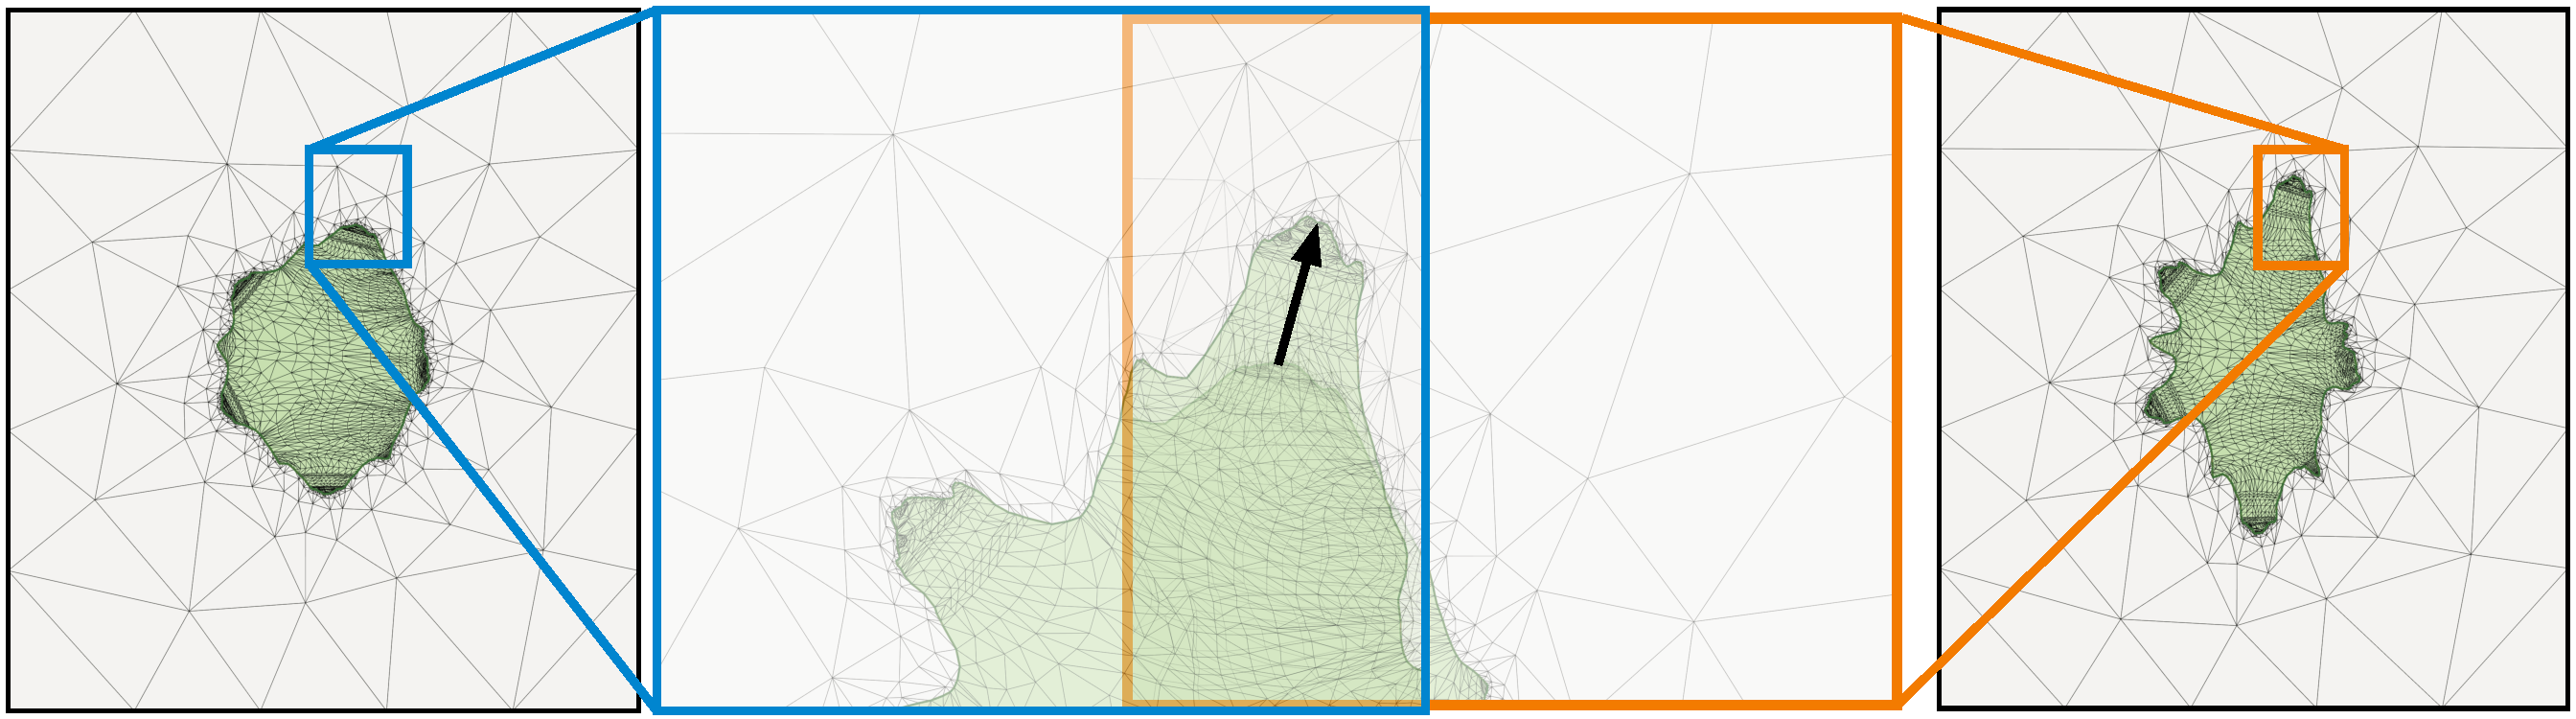
\includegraphics[width=\columnwidth]{scaf-tex/figs/camel_step.pdf}
\caption{A single iteration of our algorithm (from left to right) drastically reduces the distortion. The black vector in the center is ~150 times longer than the average edge length of its 1-ring. Iterative methods would need thousands of iterations to achieve a similar progress.}
\vspace{-0.3cm}
\label{scaf:fig:largestep}
\end{figure}

% what about... the original is convoluting the metric on the scaffold with the independence to orientation
Despite the orientation-dependent box used as scaffold boundary, our optimization produces results that are, in practice, independent of orientation.  We show this effect in Figure~\ref{scaf:fig:random-rotate} where we initialize the optimization with 1000 randomly rotated Tutte's mappings of the same camel model and run our optimization.  The isometric distortion of the model after 50 iterations is quite similar in all trials (the minimum, maximum, average, standard deviation of distortion errors in all 1000 runs are 0.1086, 0.1107, 0.1095, 3.2698e-4 resp.) indicating very little change based on the initial orientation.
%Since we enforce an isometric energy to the scaffold, translation and rotation is encouraged to make space for 

\begin{figure}[t]
\centering
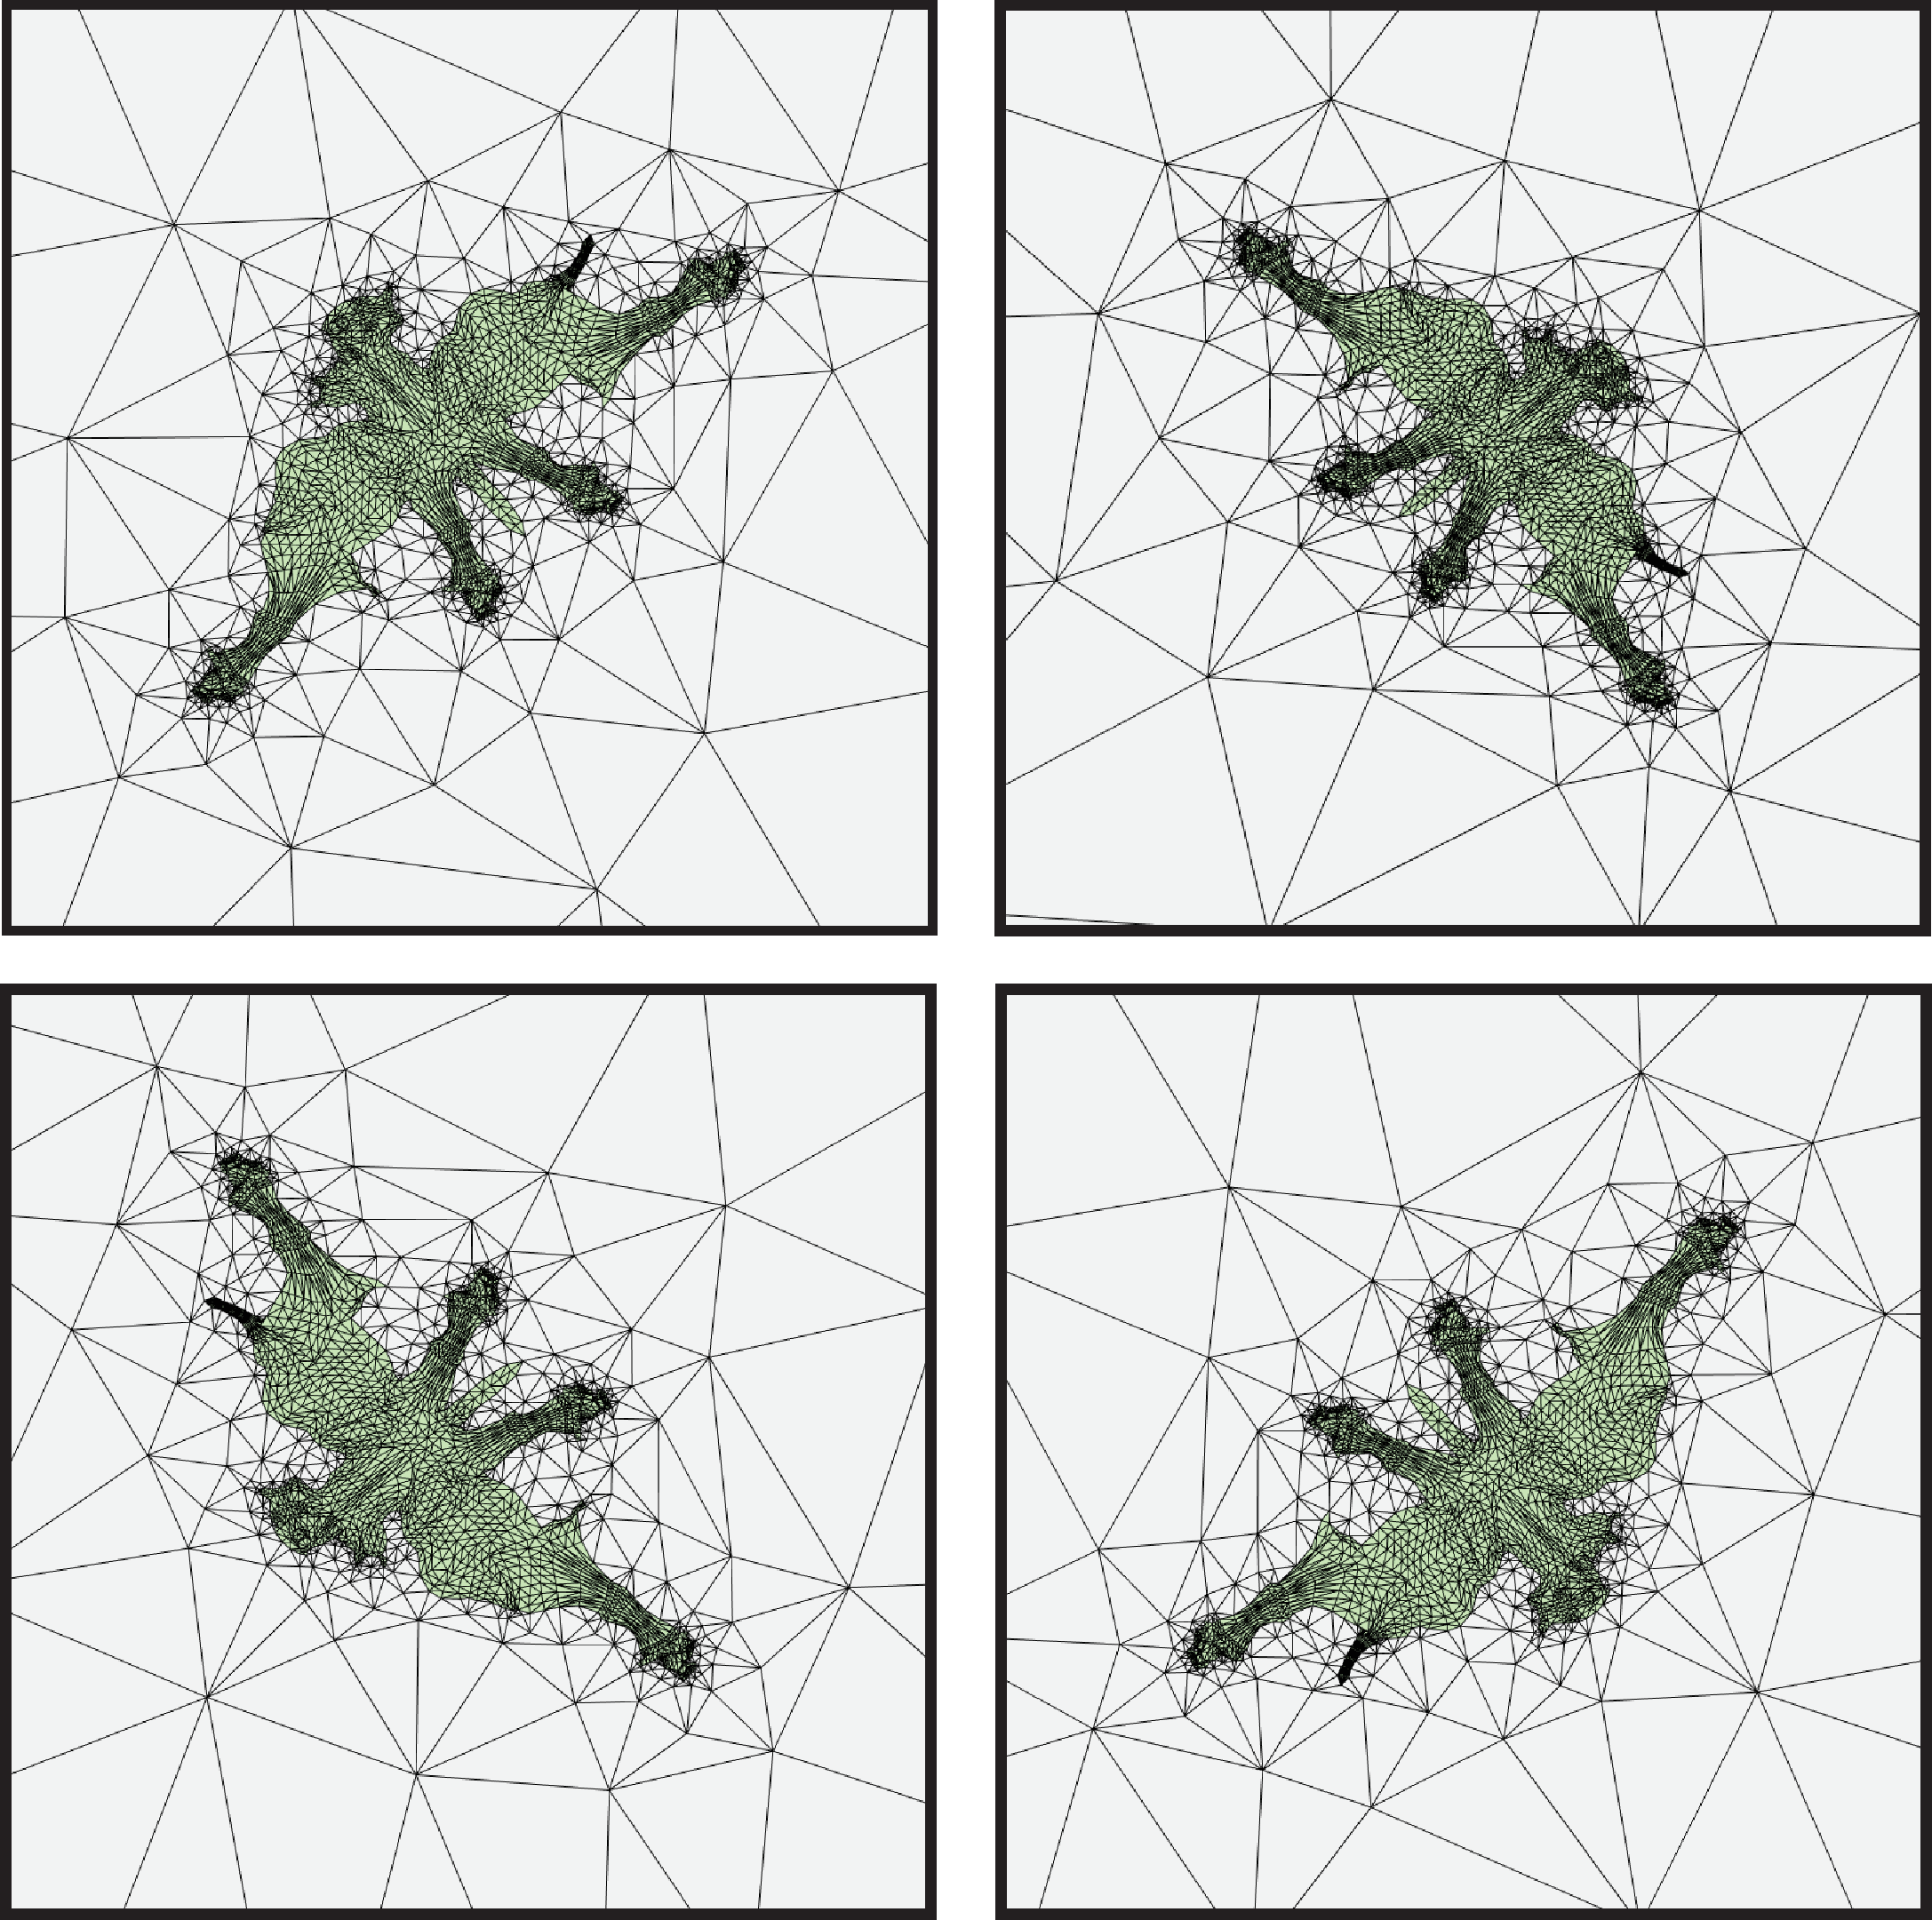
\includegraphics[width=\columnwidth]{scaf-tex/figs/random-rotate.pdf}
\caption{
{Our algorithm is independent to the initial orientation. We rotate the initializing Tutte's mapping of the camel model and obtain results with similar isometric distortion.}}
\vspace{-0.2cm}
\label{scaf:fig:random-rotate}
\end{figure}


\paragraph{Timings} The timings for all the results in the paper are reported in Table \ref{tab:timings}.
\begin{table}[t]
	\centering
	\begin{adjustbox}{width=\columnwidth,totalheight=\textheight,keepaspectratio}
	\begin{tabular}{llrrrrrrr}
%		\hline
\textbf{{Type}} &\textbf{Model} & $\mathbf{\#V}$	& $\mathbf{\#F}$ & $\mathbf{\#V_S}$	& $\mathbf{\#F_S}$ & \textbf{It.} & \textbf{{Total Time (s)}} & \textbf{{It. Time (s)}}\\
\hline
\multirow{2}{*}{Atlas}&Nefertiti (Fig.~\ref{scaf:fig:teaser})
&1697	&2823	&983/	247&	1945	/728&	50&	0.71&0.01\\
&Maneki-Neko (Fig.~\ref{scaf:fig:packing2D})
&23025	&43648	&2427	/725&	7174/	3770&	50&	16.81&0.34\\
\hline
\multirow{12}{*}{2D}
&Hand (Fig.~\ref{scaf:fig:different_weight})
&2239&4046&347/280&1104/970&7&0.14&0.02\\
&Spiral (Fig.~\ref{scaf:fig:recovering})
&54&52&78/36&190/106&50(50)&0.04(0.21)&0.01\\
&Thai Statue (Fig.~\ref{scaf:fig:miq_database}, left)
&42405&79970    &   3665/1593&12148/8004&50&28.28&0.56\\
&Filigree (Fig.~\ref{scaf:fig:miq_database}, right)
&56062&100000&9160/2627&30422/17356&100&75.99&0.76\\
&Lucy (Fig.~\ref{scaf:fig:scalability})&	501105&	1000000&	1856/	3470&	5900/	5674&	100&	2524.22&25.24\\
&Lucy (Fig.~\ref{scaf:fig:scalability})&	1001375&	1999999&	2284/	4400&	7297/	7133&	100&	7251.00&72.51\\
&Lucy (Fig.~\ref{scaf:fig:scalability})&	2002031&	3999999&	3587/	6930&	11215/	10985&	100&	22500.07&225.00\\
&Lucy (Fig.~\ref{scaf:fig:scalability})&	3002899&	5999999&	5135/	9859&	16047/	15601&	100&	52235.31&522.35\\
&Lucy (Fig.~\ref{scaf:fig:scalability})&	4002816&	8000000&	5140/	10288&	15890/	15918&	100&	59413.14&594.13\\
&Lucy (Fig.~\ref{scaf:fig:scalability})&	5003408&	10000000&	6194/	12231&	19182/	19040&	100&	95247.59&952.47\\
&Lucy (Fig.~\ref{scaf:fig:scalability})&6004111&12000000 & 7357/6418 & 2291/21036 &50 & 78726.05 &1574.52\\
&Animal (Fig.~\ref{scaf:fig:manuallycut})
&19937&39040&747/593&2306/1998&50&15.36&0.31\\
&Space Filling (Fig.~\ref{scaf:fig:smith})
&79545&146832&90815/88237&181608/176452&200(250)&547.13(1836.58)&5.30\\
&Horse (Fig.~\ref{scaf:fig:smith-all}) & 20636 & 39698 & 1343/984 & 4238/3520 & 30(10) & 8.26(12.03) & 0.28(1.20) \\
&Camel (Fig.~\ref{scaf:fig:smith-all}) & 2032 & 3576 & 384/272 & 1234/1010 & 30(10) & 0.52(1.13) & 0.02(0.11) \\
&Cow (Fig.~\ref{scaf:fig:smith-all}) & 3195 & 5804 & 491/277 & 1546/1118 & 30(10) & 0.81(1.74) & 0.03(0.17) \\
&Tricera (Fig.~\ref{scaf:fig:smith-all}) & 3163 & 5660 & 544/329 & 1732/1302 & 30(10) & 0.83(1.77) & 0.03(0.18) \\
\hline

\multirow{2}{*}{3D}&Leg (Fig.~\ref{scaf:fig:flow})
&6617&13230&5016/5021&68521/68544&500&3251.17&6.50\\
&Bunny (Fig.~\ref{scaf:fig:rabbit})
&568&1132&683/706&6209/6289&50&7.16&0.14\\

\hline
	\end{tabular}
	\end{adjustbox}
			\caption{Timings and statistics for the models shown in the paper. From left to right: number of input vertices and simplices, number of initial/final scaffold vertices and simplices, number of iterations, running time in seconds. The numbers in parenthesis refer to the Newton optimization. Note that our timings are considerably higher than those reported in the SLIM paper for the Lucy model since we used the reference implementation in \protect\cite{libigl}, which {does not use} a multi-threaded solver.}
	\label{tab:timings}
	\vspace{-0.2cm}
\end{table}

